\documentclass[11pt,a4paper]{article}
\usepackage{graphicx}
\usepackage[utf8x]{inputenc}
\usepackage{titling}
\usepackage{afterpage}
\usepackage[italian]{babel}
\newcommand{\subtitle}[1]{%
\posttitle{\par\end{center}
\begin{center}\large#1\end{center}
\vskip0.5em}
}

\begin{document}
\begin{titlepage}
\title{\LARGE{}}
\subtitle{\textbf{RELAZIONE SEMESTRALE DI LABORATORIO}}
\author{Cavuoti Lorenzo, Di Meglio Francesco Paolo, Draetta Silvio, \\Geroni Francesco, Sacco Francesco}
\date{}
\maketitle
\end{titlepage}
\thispagestyle{empty}
\mbox{}
\title{\textbf{Analisi del comportamento di un LED}}
\date{}
\maketitle
\section{Introduzione}
	L'obiettivo dell'esperienza consiste nel verificare che un LED si comporti come un diodo e rispetti la legge di Shockley.

\section{Cenni Teorici}
	LED è acronimo di Light Emitting Diode. Un diodo è un elemento circuitale non ohmico (ossia non segue la legge di Ohm $V=IR$). Il suo comportamento è descritto dall'equazione di Shockley:

\begin{equation}
	\label{shockley}
	I=I_0(e^{-\frac{\Delta V}{\eta V_T}}-1)
\end{equation}

$I_0$ è l'intensità corrente di saturazione inversa, $\eta$ è un coefficiente che dipende dal diodo e $V_T$ è una differenza di potenziale termica ($V_T = \frac{k_B T}{e}$).
Tale relazione ci mostra come l'andamento dell'intensità di corrente sia non lineare.

\section{Apparato Sperimentale}
\begin{itemize}
	\item LED rosso;
	\item Scheda arduino;
	\item 2 resistenze ($R_1=68.5\pm0.6$  $\Omega$ e $R_2=671\pm 5$ $\Omega$ rispettivamente);
	\item Condensatore ($470\pm20 \%$ $\mu F$);
	\item Multimetro digitale; 
	
\end{itemize}


\section{Procedimento}
	Nel circuito rappresentato in figura (\ref{fig:circuito}) l'arduino genera un'onda quadra. Collegato all'arduino è assemblato un integratore con frequenza di taglio ($f_\tau = \frac{1}{2\pi R_1 C}$) pari a $4.9\pm 1.0$ Hz.\\
	Grazie a tale configurazione il segnale alternato viene trasformato in uno continuo, che rappresenta il segnale in ingresso nel LED.
	Per verificare la legge di Shockley sono necessarie le misure di differenza di potenziale ai capi del LED e di intensità di corrente che vi passa. \\
	La misura dell'intensità di corrente viene effettuata ponendo prima del LED la resistenza $R_2$ e misurando ai suoi capi la differenza di potenziale tramite l'arduino (in particolare questo misura le differenze di potenziale prima e dopo la resistenza in modo separato; i valori di d.d.p. sono a terra). Sfruttando la legge di Ohm è poi possibile ottenere il valore d'intensità di corrente cercato.
	\subsection{Calibrazione di arduino}
		Le misure di differenza di potenziale che arduino restituisce non sono calibrate: queste infatti sono numeri interi compresi tra 0 e 1023 (in unità di digitalizzazione, dette digit), dove lo 0 rappresenta una d.d.p. nulla e 1023 la massima fornita dalle uscite digitali di arduino.
		Chiamando quest'ultima $V_{ref}$ e misurandola col multimetro digitale ($5.08 \pm 0.03 \ $V), si definisce $\xi = {V_{ref}}/1023$ come fattore di calibrazione. La tensione in volt è quindi esprimibile dal prodotto di $\xi$ e il valore in digit della stessa.
		
		
	
\begin{figure}[h!]
	\centering
	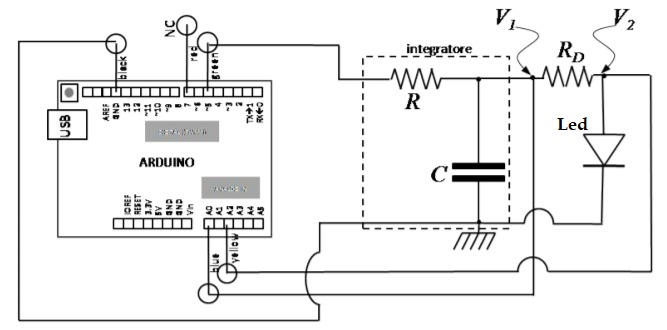
\includegraphics[width=1\linewidth]{circuitoled.png}
	\caption{Schema circuitale dell'esperienza.}
	\label{fig:circuito}
\end{figure}

\newpage

\section{Analisi dati}
	 \`{E} stato realizzato un best fit dei 256 dati, acquisiti con arduino, dell'intensità di corrente in funzione della differenza di potenziale. \`{E} stata utilizzata la funzione \verb curve_fit \ del pacchetto \verb scipy \ di Python adottando come modello la (\ref{shockley}). I parametri liberi sono $I_0$ e $\eta V_T$.
\begin{figure}[b!]
	\centering
	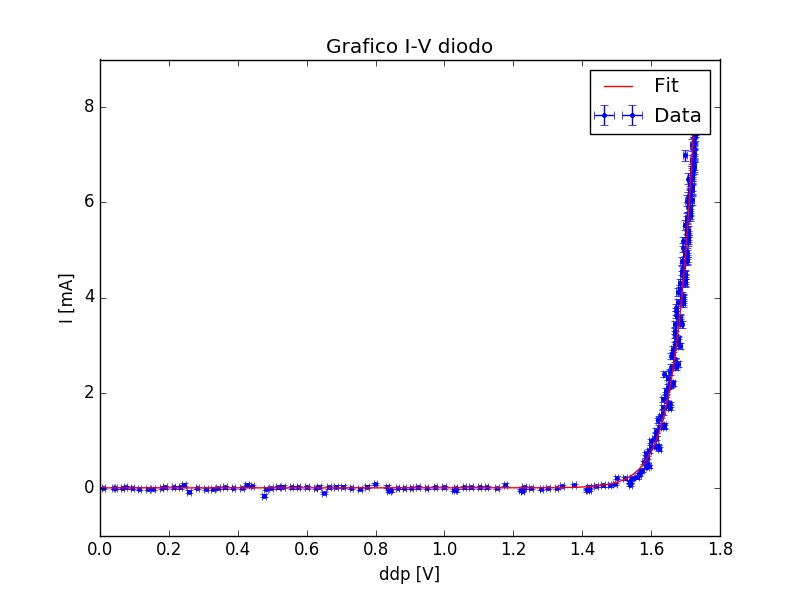
\includegraphics[width=1\linewidth]{grafico.png}
	\caption{Curva I-V LED}
	\label{fig:LED}
\end{figure}
\begin{figure}
	\centering
	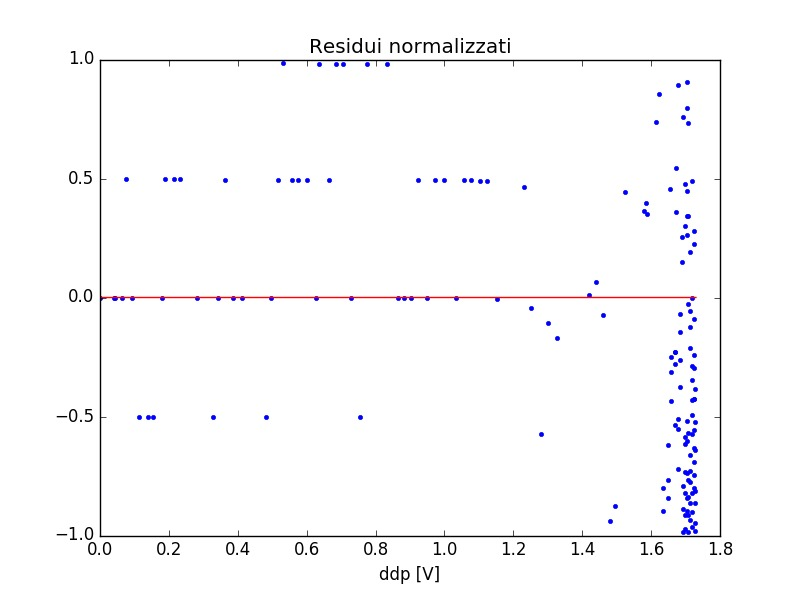
\includegraphics[width=1\linewidth]{residui.png}
	\caption{Residui normalizzati}
	\label{fig:residui}
\end{figure}
	\\ I seguenti sono i risultati del best fit, per il quale \`{e} stata usata l'opzione \verb absolute_sigma \ \verb =  \verb False ,\ poich\`{e} le acquisizioni di arduino hanno un carattere prevalentemente non statistico a causa di errori sistematici di calibrazione. 
	
	\begin{equation}
	I_0 = (8 \pm 3)\times 10^{-8} \ \textrm{nA}  
	\label{I0} 
	\end{equation}
	\begin{equation}
	\eta V_T = (53.6 \pm 0.7) \ \textrm{mV} 
	\label{nvt} 
	\end{equation}
	\begin{equation}
	\textrm{cov.\ norm.} = 0.999 
	\label{cov}
	\end{equation}
	\begin{equation}
	\chi^{2}/\textrm{ndof} = 576/254 = 2.26
	\label{chi2}
	\end{equation}
	
\section{Conclusioni}
	Da una prima osservazione dei dati si pu\`{o} gi\`{a} notare un andamento esponenziale che \`{e} quello atteso in base all'equazione (\ref{shockley}).\\
	Il valore della covarianza normalizzata (\ref{cov}) \`{e} conseguenza del modello (\ref{shockley}): se si considerano punti sperimentali in cui la parte esponenziale prevale sull'unit\`{a}, c'\`{e} una fortissima correlazione tra $I_0$ e $\eta V_T$. \\
	Il valore contenuto nella (\ref{nvt}) \`{e} ragionevolmente compatibile con l'aspettativa di circa 52 mV. Il valore della corrente di saturazione inversa (\ref{I0}) (massimo 10 $\mu A$ secondo il datasheet) \`{e} molto inferiore a quello di un comune diodo che si trova in laboratorio (circa 8 ordini di grandezza). Questo pu\`{o} spiegare il motivo per cui la crescita esponenziale (tensione di soglia) si nota a circa 1.6 V (rispetto ai circa 0.5 - 0.6 V del diodo). Inoltre, secondo datasheet, tale valore per un LED rosso \`{e} di circa 1.8. \\
	Analizzando infine il grafico (\ref{fig:residui}) si nota un pattern dovuto probabilmente all'aquisizione digitale di arduino. Tale fenomeno però diventa meno evidente da 1.2 V in poi, fino al punto in cui, circa in corrispondenza della tensione di soglia, \`{e} quasi del tutto assente. La densit\`{a} di dati presenti tra 1.6 V e 1.8 V \`{e} giustificabile dal fatto che la derivata prima dell'equazione (\ref{shockley}) cresce esponenzialmente in tale intervallo.
	In conclusione, dopo aver analizzato i dati raccolti, è possibile affermare che un led si comporti effettivamente come un diodo.
	 
	

\end{document}